% Part: model-theory
% Chapter: interpolation
% Section: separation

\documentclass[../../../include/open-logic-section]{subfiles}

\begin{document}

\olfileid{mod}{int}{sep}

\section{\printtoken{P}{sentence}નું પૃથક્કરણ}

અંતર્વેશન પ્રમેયની સાબિતી તરફ આગળ વધતાં પહેલાં થોડી પૂર્વતૈયારી
જરૂરી છે. $!A$ અને~$!B$નો અંતર્વેશક એવું !!a{sentence}~$!C$ છે કે
$!A \Entails !C$ અને $!C \Entails !B$. પ્રતિપક્ષનથી, પછીનું નિવેદન
$\lnot !B \Entails \lnot !C$ હોય ત્યારે અને માત્ર ત્યારે સાચું છે.
આ ગુણધર્મ ધરાવતું !!^a{sentence}~$!C$, $!A$ અને $\lnot !B$ને
\emph{પૃથક કરે છે} તેમ કહેવાય છે. તેથી $!A$ અને~$!B$નો અંતર્વેશક
શોધવો એટલે $!A$ અને $\lnot !B$ને પૃથક કરતું !!a{sentence} શોધવું.
ઘણી વાર થાય છે તેમ, અહીં પણ તેના સામાન્યીકરણનો વિચાર ઉપયોગી થશે:
!!{sentence}sના બે \emph{ગણો}ને પૃથક કરતું વિધાન.

\begin{defn}
વિધાન~$!C$, વાક્યોના ગણો~$\Gamma$ અને~$\Delta$ને ત્યારે અને
માત્ર ત્યારે \emph{પૃથક કરે છે} જ્યારે $\Gamma \Entails !C$ અને
$\Delta \Entails \lnot !C$. જો આવું કોઈ !!{sentence} ન હોય, તો
$\Gamma$ અને~$\Delta$ \emph{અપૃથક્કરણીય} છે.
\end{defn}

$\Gamma$, $\Delta$ અને~$!C$ના નિદર્શોના વર્ગો વચ્ચેના સમાવેશ-સંબંધો
નીચે દર્શાવ્યા છે:
\begin{figure}[h]
  \centering
  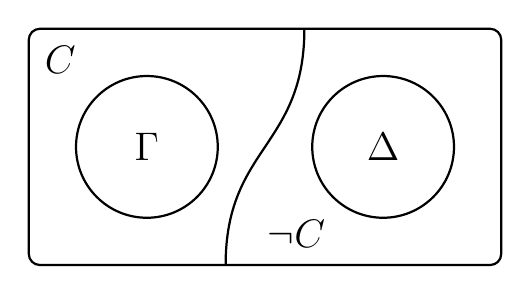
\begin{tikzpicture}[node distance=2cm, auto, thick]
    \draw [rounded corners] (0,0) -- (6,0) -- (6,3) -- (0,3) --  cycle;
    \draw (1.5,1.5) circle (0.9cm);
    \draw (4.5,1.5) circle (0.9cm);
    \path node at (1.5,1.5) {\Large $\Gamma$};
    \path node at (4.5,1.5) {\Large $\Delta$};
    \path node at (0.4,2.6) {\Large $\formula{C}$};
    \path node at (3.4,0.4) {\Large $\lnot \formula{C}$};
    \draw (2.5,0) .. controls (2.5,1.5) and (3.5,1.5) .. (3.5,3);
  \end{tikzpicture}
  \caption{$!C$, $\Gamma$ અને~$\Delta$ને પૃથક કરે છે}
  \ollabel{fig:sep}
\end{figure}


\begin{lem}\ollabel{lem:sep1}
ધારો કે $\Lang{L}_0$ એ એવી ભાષા છે જેમાં $\Gamma$ અને~$\Delta$
\emph{બંને}માં આવતા દરેક !!{constant}, !!{function} અને !!{predicate}
($\doteq$ સિવાયના) છે, અને $n\ge 0$ માટે અનંત નવા !!{constant}s
$\Obj c_n$ ઉમેરીને $\Lang{L}'_0$ મેળવાય છે. તો જો $\Gamma$ અને
$\Delta$, $\Lang{L}_0$માં અપૃથક્કરણીય હોય, તો તેઓ $\Lang{L}'_0$માં
પણ અપૃથક્કરણીય છે.
\end{lem}

\begin{proof}
આપણે પરોક્ષ રીતે આગળ વધીએ: વિરોધાભાસ માટે ધારો કે $\Gamma$ અને
$\Delta$, $\Lang{L}'_0$માં પૃથક્કરણીય છે. તો કોઈ $!C\in\Lang{L}_0$
માટે $\Gamma \Entails \Subst{!C}{c}{x}$ અને $\Delta \Entails \lnot
\Subst{!C}{c}{x}$ (અહીં $c$ નવો !!{constant} છે---$!C$માં આવા એકથી
વધુ નવા !!{constant} હોય તે કિસ્સો સમાન છે). સઘનતાથી, $\Gamma$નો
કોઈ \emph{સાન્ત} ઉપગણ~$\Gamma_0$ અને $\Delta$નો કોઈ \emph{સાન્ત}
ઉપગણ~$\Delta_0$ એવા છે કે $\Gamma_0 \Entails \Subst{!C}{c}{x}$ અને
$\Delta_0 \Entails \lnot \Subst{!C}{c}{x}$. $\Gamma_0$નાં બધાં
!!{formula}sના સંયોજનને~$!G$ અને $\Delta_0$નાં બધાં !!{formula}sના
સંયોજનને~$!H$ કહો. તો
\begin{align*}
  !G & \Entails \Subst{!C}{c}{x}, & !H  \Entails \lnot \Subst{!C}{c}{x}.
\end{align*}
પહેલામાંથી સર્વત્રીકરણ વડે $!G \Entails \lforall[x][!C]$ મળે છે;
બીજામાંથી પ્રતિપક્ષન વડે $\Subst{!C}{c}{x} \Entails \lnot !H$, અને
તેથી $\lforall[x][!C] \Entails \lnot !H$ પણ મળે છે. ફરી પ્રતિપક્ષનથી
$!H \Entails \lnot \lforall[x][!C]$. એકદિશવર્ધિતાથી,
\begin{align*}
  \Gamma &\Entails \lforall[x][!C], &
  \Delta & \Entails \lnot \lforall[x][!C],
\end{align*}
અને તેથી $\lforall[x][!C]$, $\Gamma$ અને~$\Delta$ને $\Lang{L}_0$માં
પૃથક કરે છે.
\sourcecorrection{OLINT-001}{સ્થિર અંગ્રેજી મૂળની
  \texttt{separation.tex}, પંક્તિ~75માં પૂર્વધારણા~$!H$ના સ્થાને
  અગાઉ ક્યાંય વ્યાખ્યાયિત ન થયેલું~$\delta$ આવે છે. પ્રતિપક્ષનથી
  મેળવવાના નિષ્કર્ષમાં અહીં $\lnot !H$ પુનઃસ્થાપિત કર્યું છે.}
\end{proof}

\begin{lem}\ollabel{lem:sep2}
ધારો કે $\Gamma \cup \{ \lexists[x][!S] \}$ અને~$\Delta$
અપૃથક્કરણીય છે, અને $c$ એવો નવો !!{constant} છે જે $\Gamma$,
$\Delta$ કે~$!S$માં આવતો નથી. તો $\Gamma \cup \{ \lexists[x][!S],
\Subst{!S}{c}{x} \}$ અને~$\Delta$ પણ અપૃથક્કરણીય છે.
\end{lem}

\begin{proof}
વિરોધાભાસ માટે ધારો કે $!C$, $\Gamma \cup \{ \lexists[x][!S],
\Subst{!S}{c}{x}\}$ અને~$\Delta$ને પૃથક કરે છે, જ્યારે $\Gamma \cup
\{\lexists[x][!S] \}$ અને~$\Delta$ અપૃથક્કરણીય છે. આપણે બે કિસ્સા
પાડીએ છીએ:
\sourcecorrection{OLINT-002}{સ્થિર અંગ્રેજી મૂળની
  \texttt{separation.tex}, પંક્તિ~95માં $\lexists$ના સૂત્ર-દલીલખંડને
  જરૂરી ચોરસ કૌંસને બદલે વાંકિયા કૌંસમાં મૂક્યો છે; તેથી તે
  ક્વાન્ટિફાયરના વ્યાપ તરીકે લેવાતો નથી. અહીં
  \texttt{\string\lexists[x][!S]} પુનઃસ્થાપિત કર્યું છે.}
\begin{enumerate}
\item $c$, $!C$માં આવતો નથી: આ કિસ્સામાં $\Gamma \cup
  \{\lexists[x][!S], \lnot!C \}$ સંતોષ્ય છે (નહિતર $!C$, $\Gamma
  \cup \{\lexists[x][!S] \}$ અને~$\Delta$ને પૃથક કરે). તેમાં
  $\Subst{!S}{c}{x}$ ઉમેર્યા પછી પણ તે સંતોષ્ય રહે છે, તેથી અંતે
  $!C$, $\Gamma \cup \{ \lexists[x][!S], \Subst{!S}{c}{x} \}$ અને
  $\Delta$ને પૃથક કરતું નથી.
\item $c$, $!C$માં આવે છે, જેથી $!C$નું સ્વરૂપ
  $\Subst{!C}{c}{x}$ છે. ત્યારે
  \[
  \Gamma \cup \{ \lexists[x][!S], \Subst{!S}{c}{x}\} \Entails \Subst{!C}{c}{x},
  \]
  અને તેથી નિગમન પ્રમેય તથા સર્વત્રીકરણ વડે
  $\Gamma, \lexists[x][!S] \Entails \lforall[x][(!S \lif !C)]$,
  અને છેવટે $\Gamma \cup \{ \lexists[x][!S] \} \Entails
  \lexists[x][!C]$. બીજી તરફ, $\Delta \Entails \lnot
  \Subst{!C}{c}{x}$ અને તેથી સર્વત્રીકરણ વડે $\Delta \Entails \lnot
  \lexists[x][!C]$. એટલે $\Gamma \cup \{\lexists[x][!S] \}$ અને
  $\Delta$ પૃથક્કરણીય છે, જે વિરોધાભાસ છે.
\end{enumerate}
\end{proof}

\end{document}
